%!TEX root = ../deco_star.tex


%-------------------------------------------------------------------------
%-------------------------------------------------------------------------
\section{Taxonomy of Control Mechanisms}\label{sec:taxo_control_mechanism}

The following taxonomy lays groundwork for our later evaluation of control mechanisms of the state of the art. It is difficult to derive the discussion of creative means directly from the related work, as its authors have followed different motivations and have emphasized various aspects when describing their work and results. To classify the work in an objective and unified manner, we analyze general characteristics of control with digital creation tools and relate the actual presented control mechanisms to them. Based on this analysis, we then review the related work in~\Cref{sec:analysis}.

\newcommand{\controlParamsFigWidth}{0.9}

\subsection{Control Characteristics}\label{control_charateristics}
A creation process can be described by answering the questions of \textit{how}, \textit{what}, \textit{where}, \textit{when} and \textit{who}. These characteristics can be discussed in various creation contexts and could even be translated to traditional media such as aquarell on paper.

\noindent\textbf{How (User Interaction)} is a control executed or an input given by an artist? How \refremove{}{far}\rev{}{detached} is it from the visual result on the canvas? 

\begin{figure}[H]
    \centering
        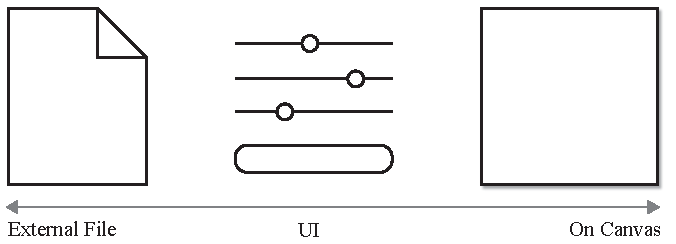
\includegraphics[width=\controlParamsFigWidth\linewidth]{figures/control_paradigms/how.pdf}
    % \caption{How is input given?}
\end{figure}

\begin{itemize}
    \item \textit{File}: The control is externally given, such as with code or a configuration file.
    \item \textit{UI}: A separate UI is given through which an artist gives input and activates states. UIs are often in close proximity to the canvas, carefully designed and easily usable. However, because they detach the work from the actual output, UIs have an abstract nature \rev{}{of indirection}. An artist must actively translate the interaction with the UI to the resulting output on the canvas.
    \mf{I would propose to \emph{always} use “separate UI” instead of “UI”. Outside our field, both external files and on-canvas techniques constitute possible interfaces}
    \item \textit{On canvas}: Controls are executed directly on the output canvas. Most of them require an activation or selection of a tool in a separate UI, such as selecting a pen for drawing on a canvas. 
    There are cases where controls cannot clearly be classified as either UI or on canvas. A pen, for example, can have different characteristics that an artist needs to set in the UI. The adjustment of settings should be as seamlessly integrated into an on-canvas tool as possible (\eg with choices appearing as tool tips). 
\end{itemize}


\noindent\textbf{What (Content)} does an artist give as input? What is the level of abstraction of the content that an artist works with?
\begin{figure}[H]
    \centering
        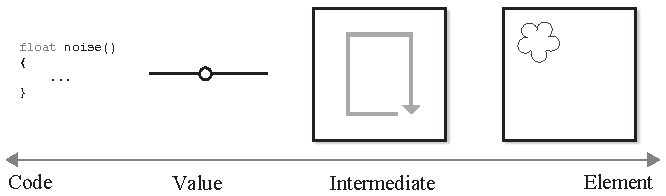
\includegraphics[width=\controlParamsFigWidth\linewidth]{figures/control_paradigms/what.pdf}
        % \caption{What does an artist give as input?}
\end{figure}

\begin{itemize}
    \item \textit{Code}: Input is a syntactically structured formal language.
    \item \textit{Value}: The input is a single value, chosen from a range - for example, with a slider.
    \item \textit{Intermediate}: The input is visual but of an abstract nature, such as controlling sketches for a mask or arrows for directionality. Artists still have to interpret how the inputs affect the result.
    \item \textit{Element}: The input is a component of the resulting pattern.
\end{itemize}

\noindent\textbf{Where (Canvas)} has the input an effect spatially and what is the area of influence? 

\mf{In the current revision, the where-picture floats into the when-block, which disturbs the reader. 
If this happens in the final version, I propose to drop the figure-environment and place it here with a brutal
includegraphics inside a centering block, see comment in code.}
%
% Mind the gap: needs a separate paragraph, otherwise, centering affects previous text as well.
%
%{\centering
%        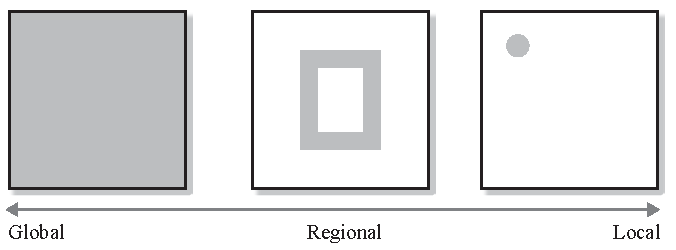
\includegraphics[width=\controlParamsFigWidth\linewidth]{figures/control_paradigms/where.pdf
%
%
%}
\begin{figure}[hbt]
    \centering
        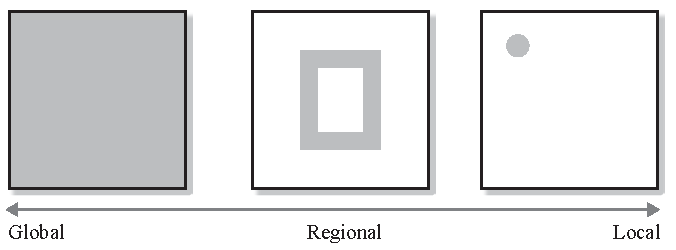
\includegraphics[width=\controlParamsFigWidth\linewidth]{figures/control_paradigms/where.pdf}
        % \caption{Where does the input have an effect?}
\end{figure}

The input can have \textit{global} influence, \textit{regional}, \eg~on a drawn curve or \textit{local}, \eg~on one specific element.



\textbf{When (Timeline)} is the input given and at what time in the creation process is the control executed? 
\begin{figure}[H]
    \centering
        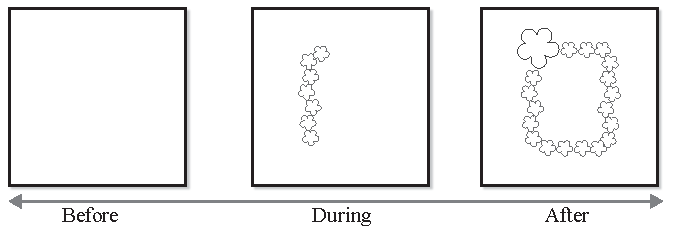
\includegraphics[width=\controlParamsFigWidth\linewidth]{figures/control_paradigms/when.pdf}
        % \caption{When is the input given?}
\end{figure}

Input can be given \textit{before}, \textit{during} the creation process, when parts of the results are already visible \eg~with a painting mechanism, or \textit{after} the creation process. The result is visible to the artist and can be adjusted retrospectively.


\noindent\textbf{Who (User)} gives the input in regard to the needed type of skill set. 
\begin{figure}[H]
    \centering
        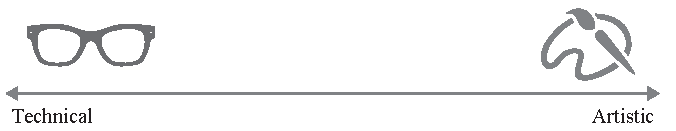
\includegraphics[width=\controlParamsFigWidth\linewidth]{figures/control_paradigms/who.pdf}
        % \caption{Who can give the input? Which skill set is needed?}
\end{figure}

This category can be in part derived from the above characteristics of \textit{how} and \textit{what}. In most general terms, this category can be classified the skill set of a \textit{Programmer}, for giving, \eg~code as input, requiring analytical-formal and logical thinking and the ability to abstract. On the other end of the spectrum, the skill set of an \textit{Artist} is needed, \eg~for drawing, requiring intuitive-visual and spatial thinking and the ability to create. The \textit{who} category is listed here for completeness. \revremove{}{However, to answer questions of}\rev{}{The discussion of} needed competencies, skill\rev{}{s}\revremove{}{-}s and mindsets, including the accompanying psychological and artistic aspects, is out of the scope of this survey\rev{}{, though}.

\subsection{Control Mechanisms}\label{subsec:taxo_control_mechanism}
Next to the above overall relevant factors for an artist using digital tools, we now classify the control mechanisms as they are described in the state of the art. These low-level mechanisms define what an artist can (or has to) work with and are specified for each reference in Table~\ref{table:analysis}. Because this survey focuses on interfacing algorithms, UI specifics, such as the layout of buttons, are not considered. For each mechanism we summarize the \textit{how}, \textit{what}, \textit{where} and \textit{when} characteristics over all reviewed publications and with that show the connections and capabilities of the different control mechanisms and potential trade-offs between approaches in Table~\ref{table:taxo_controlmechanism}.

\noindent\textbf{Initialization}
\begin{itemize}
    \item \textit{System Configuration}: Required overall setup of the system, such as computing caches or training a model. This is usually a one-time investment.
    \item \textit{Task Initialization}: A non-creative task that has to be executed each time in order to produce an output, such as selecting the specific optimization algorithm.
\end{itemize}

\noindent\textbf{Exemplars}
\begin{itemize}
    \item \textit{Image}: An example image that should be matched in its entirety. Examples are usually pixel data.
    \item \textit{Element Arrangement}: An example element arrangement that should be matched in its entirety. Elements are usually separate shapes and might carry additional data.
    \item \textit{Element}: One specific, individual, asset that becomes in the result part of a whole. Elements can be shapes or pixel data.
\end{itemize}

\noindent\textbf{Parameterization}
\begin{itemize}
    \item \textit{Visual Output}: Parameters that can adjust visual features directly in the output.
    \item \textit{System/Generation}: Parameters that influence the output indirectly, such as parameters for an optimization algorithm or constraints.
\end{itemize}

\noindent\textbf{Handling}
\begin{itemize}
    \item \textit{Visualization}: Any type of visual interface that goes beyond the standard UI elements, such as sliders and buttons.
    \item \textit{Image-Based}: Images as indirect control input, such as pixel data masks.
    \item \textit{Sketch-Based}: Sketches and curves directly put on the canvas - for example, the drawing of a mask with a pen tool.
\end{itemize}

\noindent\textbf{Filling}
\begin{itemize}
    \item \textit{Shapes}: A space to fill (\eg~a specific shape).
    \item \textit{Masking}: Areas within the shape to fill that should remain unaffected.
    \item \textit{Curves to Fill}: A one-dimensional curve or path to be filled. The curve is given as a whole before the filling starts.
    \mf{Can you actually “fill” a (1D) curve? Should we say: “follow a curve” instead?}
\end{itemize}

\noindent\textbf{Guiding}
\begin{itemize}
    \item \textit{Brushing/Strokes to Follow}: A curve, usually created by mouse movements or with a stylus pen, that is filled with output elements -often understood as brushing.
    \item \textit{Directions}: Visual elements such as intermediate curves, arrows or output components that define directions for the design to follow (\eg~with an underlying vector field).
\end{itemize}

\noindent\textbf{Placing}
\begin{itemize}
    \item \textit{Element Placement}: The direct placement of components on the canvas as part of the final result.
    \item \textit{Element Drag \& Drop}: Drag and drop of components on the canvas within the existing result.
\end{itemize}

